\chapter{Multi-Criteria Decision Making}

For convenience, we will use the abbreviation MCDM to refer to Multi-Criteria Decision Making throughout this chapter and the remainder of the book. This field is also commonly known as Multi-Attribute Decision Making (MADM).



\section*{Motivation}
We will start explaining the difference between Multicriteria Decision-Making (MCDM) and Multiobjective Optimization with the following problem:\\

Imagine a team working on \textnormal{sustainable building design} wants to find the best design considering only 2 variables: the amount of natural lightning and the energy efficiency. Then they model it mathematically:\vspace{-0.7em}
\begin{itemize}
    \item Both properties of a building design will be quantified with continuous real variables ranging from 0 to 5.\vspace{-0.8em}
    \item Technical limitations give a well defined feasible region.\vspace{-0.7em}
\end{itemize}
The key challenge is balancing natural lighting and energy efficiency. More natural light means we need larger windows, but this reduces the building's thermal insulation. On the other hand, smaller windows help save energy but don't let in as much daylight.\\

Formally, this is a Multiobjective Optimization Problem where we maximize two functions simultaneously: natural lighting and energy efficiency. Such problems generally do not have a unique optimal solution where both objectives reach their maximum values, but rather a set of solutions called the \textit{Pareto frontier}: a subset of feasible solutions where improving one objective necessarily requires worsening another\footnote{This condition is called Pareto Optimality.}.\\

Once the Pareto frontier has been identified
\footnote{In general, Multiobjective Optimization problems are not tractable, often involve many dimensions, and cannot be solved analytically like the simple example plotted in \ref{fig:pareto_frontier}. Common solution approaches include metaheuristic algorithms such as Goal Programming and Evolutionary Algorithms.}
(see figure \ref{fig:pareto_frontier}), it cannot be directly presented as a solution to the customer since it represents an infinite set of building designs. Therefore, the team selects 5 representative options to present to the customer. \\

This leads to a new decision problem: how should the customer choose among these 5 options? The decision requires evaluating both objective criteria (like the ones already considered but also others such as number of rooms and floor area) and subjective criteria (like aesthetic appeal and practical layout). A decision maker must determine which criteria to consider, their relative importance, and how to assess subjective attributes. This type of selection problem is what we call a MCDM problem. The options (in this case, building designs) will be assumed to be given\footnote{
In this example, we are studying an a posteriori approach, where a set of solutions is generated first and then presented to the decision maker. This is one of three main approaches along with a priori methods (where preferences are specified before generating alternatives) and interactive methods (which involve iterative preference refinement).}.

\begin{figure}[ht]
    \centering
    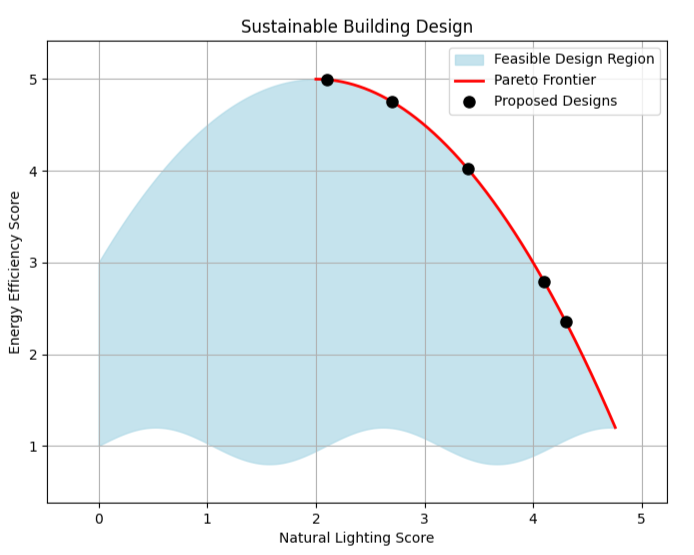
\includegraphics[width=0.6\textwidth]{ch2/figures/pareto.png}
    \caption{Pareto Frontier, feasible region and proposed designs for Sustainable Building Design}
    \label{fig:pareto_frontier}
\end{figure}

\section{Crisp MCDM Methods} \label{sec:crisp_methods}
The definitions and algorithms presented in this section are based on \cite{handbookmcdm}.\\

%Tb he leido en "lectura diagonal pag 15" sobre la clasificación en Value measurement, goal aspirations y outranking methods

\signal{From \cite{Sahoo_Goswami_2023}:}\\
\say{MCDM  methods  provide  a  systematic  and  structured framework  for  decision-making.  They  enable  decision-makers  to  break  down  complex problems  into  a  set  of  criteria,  evaluate  alternatives  against  these  criteria,  and  make informed choices based on well-defined decision rules.}
\\



% A Handbook on Multi-Attribute Decision-Making Methods, First Edition.
% Omid Bozorg-Haddad, Babak Zolghadr-Asli, and Hugo A. Loáiciga.
% © 2021 John Wiley & Sons, Inc. Published 2021 by John Wiley & Sons, Inc.

Therefore, the problem formulation usually starts by defining a decision matrix:

\begin{definition}[Decision-Matrix] 
    Let $\A =\{a_i\mid 1\leq i \leq n\} $ be the set of $n\in \N$ alternatives and $\C =\{c_j\mid 1\leq j \leq m\}$ the set of $m \in \N$ criteria. We may represent the value of the alternative $a_i$ with regard to a criterion $c_j$ as the element $d_{ij}$ of a decision-matrix $D$ as follows:
    \[D=
\setlength{\arraycolsep}{5pt} % adjust spacing if desired
\begin{array}{c@{\,}l}
  % Left block: matrix with column labels underneath
  \begin{array}{c}
    \begin{pmatrix}
      d_{11} & d_{12} & \cdots & d_{1m} \\
      d_{21} & d_{22} & \cdots & d_{2m} \\
      \vdots & \vdots & \ddots & \vdots \\
      d_{n1} & d_{n2} & \cdots & d_{nm}
    \end{pmatrix} \\[2mm] % vertical space between matrix and column labels
    \begin{array}{llll}
      \scriptstyle c_1 \hspace{1mm}& \hspace{1mm}\scriptstyle c_2 \hspace{1mm} & \hspace{1mm}\cdots  &   \hspace{1mm}\scriptstyle c_m
    \end{array}
  \end{array}
  % Right block: row labels aligned with matrix rows
  \hspace{-2.5mm}
  \begin{array}{l}
    \scriptstyle a_1 \\%[-2.5mm]
    \scriptstyle a_2 \\%[-2.5mm]
    \scriptstyle \vdots \\%[-2.5mm]
    \scriptstyle a_n\\
    \\
  \end{array}
\end{array}
\]
Where each row represents an alternative's values across all criteria, while each column shows how all alternatives perform on a single criterion.
    
\end{definition}


There is no standard classification of all the MCDM methods and there are as well mixed methods that involve ideas from a variety of them. But in order to get an approximate picture of the field, we are going to follow the classification from Belton and Stewart (2002) and see the most common methods (figure \ref{fig:MCDM_classification}):

\begin{itemize}
    \item \textbf{Value Measurement Methods:} assign each alternative a numerical value by aggregating its performance on various criteria into a single overall score, allowing for direct comparison of alternatives. They assume that all criteria can be quantified on a common scale.
    \begin{itemize}
        \item \textbf{AHP (Analytic Hierarchy Process):} Decomposes the decision problem into a hierarchical structure and uses pairwise comparisons to derive weights and scores, which are then aggregated to compute an overall value.
        \item \textbf{ANP (Analytic Network Process):} Extends AHP by accounting for interdependencies among criteria and alternatives, yet still relies on aggregating performance scores into a global value.
        \item \textbf{MAUT (Multiattribute Utility Theory):} Constructs a utility function that maps the performance of each alternative on different criteria to an overall utility value, capturing the decision maker's preferences.
    \end{itemize}
    
    \item \textbf{Goal Aspirations or Reference Level Methods:} evaluate alternatives based on their distance from pre-established ideal or reference levels. Instead of simply aggregating scores, they measure how closely each alternative meets or deviates from desired targets without requiring explicit trade-offs or weight assignments.
    \begin{itemize}
        \item \textbf{TOPSIS (Technique for Order of Preference by Similarity to Ideal Solution):} Ranks alternatives by computing their distances to both an ideal (aspiration) and an anti-ideal solution, favoring those closest to the ideal.
        \item \textbf{VIKOR (VlseKriterijumska Optimizacija I Kompromisno Resenje):}         Identifies a compromise solution by balancing the closeness of each alternative to an ideal reference point with the need to minimize regret, considering both group utility and individual dissatisfaction.
        \item \textbf{BWM (Best Worst Method):} Determines criteria weights through comparisons between the best and worst criteria against all others, thereby setting performance reference points for the evaluation.
    \end{itemize}
    
    \item \textbf{Outranking Methods:} compare alternatives pairwise to determine preference, indifference, or incomparability, leading to a ranked selection based on relative performance.
    \begin{itemize}
        \item \textbf{ELECTRE Family (Elimination and Choice Expressing Reality):}
        Uses concordance (measuring the degree of agreement) and discordance (measuring the opposition) indices in pairwise comparisons to establish if one alternative outranks another.
        \item \textbf{PROMETHEE Family (Preference Ranking Organization Method for Enrichment Evaluations):} Applies preference functions to compare alternatives pairwise, producing outranking flows that help to rank the alternatives.
    \end{itemize}
\end{itemize} 





\begin{figure}[htbp]
    \centering
    \begin{tikzpicture}[
        node distance=2cm,
        every node/.style={draw, rectangle, rounded corners, align=center, fill=blue!10, minimum width=2.5cm, minimum height=1cm},
        scale=1, transform shape
    ]
        % Root node
        \node (mcdm) {MCDM Methods};
    
        % First level: Categories arranged to the right of the root with increased vertical spacing
        \node (value) [right=3cm of mcdm, yshift=3.8cm] {Value Measurement\\Methods};
        \node (goal)  [right=3cm of mcdm] {Goal Aspirations/\\Reference Level Methods};
        \node (outrank) [right=3cm of mcdm, yshift=-3.2cm] {Outranking Methods};
    
        % Arrows from root to first-level categories
        \draw[->, thick] (mcdm) -- (value);
        \draw[->, thick] (mcdm) -- (goal);
        \draw[->, thick] (mcdm) -- (outrank);
    
        % Second level: Children of "Value Measurement Methods"
        \node (anp)  [right=2.7cm of value, yshift=1.2cm] {ANP};
        \node (ahp)  [right=2.7cm of value, yshift=0cm] {AHP};
        \node (maut) [right=2.7cm of value, yshift=-1.2cm] {MAUT};
    
        \draw[->, thick] (value) -- (anp);
        \draw[->, thick] (value) -- (ahp);
        \draw[->, thick] (value) -- (maut);
    
        % Second level: Children of "Goal Aspirations/Reference Level Methods"
        \node (topsis) [right=1.8cm of goal, yshift=1.2cm] {TOPSIS};
        \node (vikor)  [right=1.8cm of goal] {VIKOR};
        \node (bwm)    [right=1.8cm of goal, yshift=-1.2cm] {BWM};
    
        \draw[->, thick] (goal) -- (topsis);
        \draw[->, thick] (goal) -- (vikor);
        \draw[->, thick] (goal) -- (bwm);
    
        % Second level: Children of "Outranking Methods"
        \node (electre)   [right=2.5cm of outrank, yshift=0.6cm] {ELECTRE};
        \node (promethee) [right=2.5cm of outrank, yshift=-0.6cm] {PROMETHEE};
    
        \draw[->, thick] (outrank) -- (electre);
        \draw[->, thick] (outrank) -- (promethee);
    \end{tikzpicture}
    \caption{Classification of MCDM Methods following Beltan and Stewart (2002).}
    \label{fig:MCDM_classification}
    \end{figure}
    
    
    


% \subsection{Utility function methods}

% \signal{
% MAUT: ordinal utility functions and cardinal utility functions (Von Neumann-Morgenstern utility theorem)}

% \subsection{Outranking methods}
% % ===========================
% % ELECTRE I
% % ===========================
% \begin{algorithm}[H]
%     \caption{ELECTRE I Method}
%     \KwIn{Decision matrix $X=[x_{ij}]$ for $m$ alternatives and $n$ criteria, criteria weights $w_j$, concordance threshold $c^*$, discordance threshold $d^*$, and ranges $R_j$ for each criterion}
%     \KwOut{Outranking relation among alternatives and selection of the best alternatives}
%     \For{each pair of alternatives $(a,b)$}{
%         \textbf{Compute Concordance Index:}\;
%         \[
%             C(a,b) = \sum_{j \in J(a,b)} w_j, \quad \text{where } J(a,b)=\{\, j \mid x_{aj} \ge x_{bj} \,\}
%         \]\;
%         \textbf{Compute Discordance Index:}\;
%         \[
%             D(a,b) = \begin{cases}
%             \max\limits_{j \in J'(a,b)} \left( \dfrac{x_{bj}-x_{aj}}{R_j} \right), & \text{if } J'(a,b)\neq\emptyset,\\[1ex]
%             0, & \text{otherwise},
%             \end{cases}
%         \]
%         where \( J'(a,b)=\{\, j \mid x_{aj} < x_{bj} \,\}\)\;
%     }
%     \For{each pair $(a,b)$}{
%         \If{\( C(a,b) \ge c^* \) \textbf{and} \( D(a,b) \le d^* \)}{
%                 Conclude that alternative \( a \) outranks \( b \) (add an edge \( a \rightarrow b \) in the outranking graph)\;
%         }
%     }
%     Determine the kernel (set of non-dominated alternatives) or derive a ranking from the outranking graph\;
%     \Return The outranking relation and selection (or ranking) of the best alternatives\;
%     \end{algorithm}
    
% % ===========================
% % PROMETHEE II
% % ===========================
% \begin{algorithm}[H]
% \caption{PROMETHEE II Method}
% \KwIn{Decision matrix $X=[x_{ij}]$ with $m$ alternatives and $n$ criteria, criteria weights $w_j$, and parameters defining the preference functions}
% \KwOut{Complete ranking of alternatives based on net outranking flows}
% \For{each pair of alternatives $(a,b)$}{
%     \For{each criterion $j=1,\dots,n$}{
%             Compute the performance difference: 
%             \[
%             d_{j}(a,b) = x_{aj} - x_{bj}
%             \]
%             Evaluate the preference degree \( P_j(a,b) \) using the chosen preference function\;
%     }
%     Compute the aggregated preference index:
%     \[
%         \Pi(a,b) = \sum_{j=1}^{n} w_j \cdot P_j(a,b)
%     \]\;
% }
% \For{each alternative \( a \)}{
%     Compute the positive outranking flow:
%     \[
%         \phi^+(a) = \frac{1}{m-1} \sum_{b \neq a} \Pi(a,b)
%     \]\;
%     Compute the negative outranking flow:
%     \[
%         \phi^-(a) = \frac{1}{m-1} \sum_{b \neq a} \Pi(b,a)
%     \]\;
%     Compute the net flow:
%     \[
%         \phi(a) = \phi^+(a) - \phi^-(a)
%     \]\;
% }
% \Return Ranking of alternatives in descending order of \(\phi(a)\)\;
% \end{algorithm}


% \subsection{Reference point and distance-based methods}

% \begin{algorithm}[H]
%     \caption{TOPSIS Method for Multi-Criteria Decision Making}
%     \KwIn{Decision matrix $X = [x_{ij}]$ with $m$ alternatives and $n$ criteria, weights $w_j$ for each criterion}
%     \KwOut{Ranking of alternatives based on relative closeness to the ideal solution}
    
%     % Step 1: Normalize the decision matrix
%     \For{$j\leftarrow 1$ \KwTo $n$}{
%         Compute normalization factor: $d_j = \sqrt{\sum_{i=1}^{m} x_{ij}^2}$\;
%         \For{$i\leftarrow 1$ \KwTo $m$}{
%             $r_{ij} \gets \dfrac{x_{ij}}{d_j}$\;
%         }
%     }
    
%     % Step 2: Calculate the weighted normalized decision matrix
%     \For{$i\leftarrow 1$ \KwTo $m$}{
%         \For{$j\leftarrow 1$ \KwTo $n$}{
%             $v_{ij} \gets w_j \times r_{ij}$\;
%         }
%     }
    
%     % Step 3: Determine the ideal and anti-ideal solutions
%     \For{$j\leftarrow 1$ \KwTo $n$}{
%         $v_j^+ \gets \max\{v_{1j}, v_{2j}, \dots, v_{mj}\}$ \quad (if $j$ is beneficial)\;
%         $v_j^- \gets \min\{v_{1j}, v_{2j}, \dots, v_{mj}\}$ \quad (if $j$ is beneficial)\;
%         \tcp{For cost criteria, swap the definitions of $v_j^+$ and $v_j^-$}
%     }
    
%     % Step 4: Calculate separation measures for each alternative
%     \For{$i\leftarrow 1$ \KwTo $m$}{
%         $S_i^+ \gets \sqrt{\sum_{j=1}^{n} (v_{ij} - v_j^+)^2}$\;
%         $S_i^- \gets \sqrt{\sum_{j=1}^{n} (v_{ij} - v_j^-)^2}$\;
%     }
    
%     % Step 5: Calculate the relative closeness to the ideal solution
%     \For{$i\leftarrow 1$ \KwTo $m$}{
%         $C_i \gets \dfrac{S_i^-}{S_i^+ + S_i^-}$\;
%     }
    
%     % Step 6: Rank the alternatives based on $C_i$
%     \Return The alternatives ranked in descending order of $C_i$\;
%     \end{algorithm}


% % ====================================
% % 2. VIKOR Method
% % ====================================
% \begin{algorithm}[H]
%     \caption{VIKOR Method}
%     \KwIn{Decision matrix \(X = [x_{ij}]\) for \(m\) alternatives and \(n\) criteria, weights \(w_j\) for each criterion, and parameter \(v \in [0,1]\)}
%     \KwOut{Ranking of alternatives based on a compromise solution}
%     \textbf{Step 1: Determine the Best and Worst Values}\;
%     \quad \For{each criterion \(j = 1,\dots,n\)}{
%         Compute the best value: 
%         \[
%           f_j^* = \max_{i}\{x_{ij}\} \quad \text{(if maximization; use \(\min\) for minimization)}
%         \]\;
%         Compute the worst value:
%         \[
%           f_j^- = \min_{i}\{x_{ij}\} \quad \text{(if maximization; use \(\max\) for minimization)}
%         \]\;
%     }
%     \textbf{Step 2: Compute the \(S\) and \(R\) Values}\;
%     \quad \For{each alternative \(i = 1,\dots,m\)}{
%         Compute the aggregated measure:
%         \[
%            S_i = \sum_{j=1}^{n} w_j \cdot \frac{f_j^* - x_{ij}}{f_j^* - f_j^-}
%         \]\;
%         Compute the individual regret measure:
%         \[
%            R_i = \max_{j=1,\dots,n} \left[ w_j \cdot \frac{f_j^* - x_{ij}}{f_j^* - f_j^-} \right]
%         \]\;
%     }
%     \textbf{Step 3: Compute the \(Q\) Value for Each Alternative}\;
%     \quad Let 
%     \[
%     S^* = \min_{i} S_i,\quad S^- = \max_{i} S_i,\quad R^* = \min_{i} R_i,\quad R^- = \max_{i} R_i
%     \]\;
%     \quad \For{each alternative \(i = 1,\dots,m\)}{
%         Compute:
%         \[
%            Q_i = v \cdot \frac{S_i - S^*}{S^- - S^*} + (1-v) \cdot \frac{R_i - R^*}{R^- - R^*}
%         \]\;
%     }
%     \textbf{Step 4: Ranking and the Compromise Solution}\;
%     \quad Rank alternatives in ascending order of \(Q_i\)\;
%     \quad \tcp{Optionally, check for acceptable advantage and stability conditions among the top alternatives}
%     \Return Ranking of alternatives based on \(Q_i\)\;
%     \end{algorithm}



% \subsection{Pairwise comparison methods}


% % ===========================
% % ANP (Analytic Network Process)
% % ===========================
% \begin{algorithm}[H]
%     \caption{Analytic Network Process (ANP)}
%     \KwIn{A set of clusters (criteria, alternatives, etc.), pairwise comparison matrices, and information on interdependencies}
%     \KwOut{Ranking of alternatives based on final priority weights}
%     \textbf{Step 1: Network Construction}\;
%     \quad Define clusters and identify the interdependencies among them\;
%     \textbf{Step 2: Pairwise Comparisons}\;
%     \quad \For{each cluster and for each interdependency between clusters}{
%         Perform pairwise comparisons to construct local comparison matrices\;
%         Compute local priority vectors (e.g., using the eigenvector method)\;
%     }
%     \textbf{Step 3: Supermatrix Formation}\;
%     \quad Assemble all local priority vectors into the initial (unweighted) supermatrix $W$\;
%     \textbf{Step 4: Weighting the Supermatrix}\;
%     \quad Adjust $W$ by cluster weights (or inter-cluster influences) to obtain the weighted supermatrix $W'$\;
%     \textbf{Step 5: Limit Supermatrix Calculation}\;
%     \quad Raise $W'$ to a sufficiently large power until convergence, i.e., 
%     \[
%     W'^{(k)} \rightarrow W^* \quad \text{as } k \to \infty
%     \]
%     \textbf{Step 6: Derive Final Priorities}\;
%     \quad Extract the final weights for the alternatives from $W^*$\;
%     \Return Ranking of alternatives based on the final weights\;
%     \end{algorithm}


% % ====================================
% % 1. Analytic Hierarchy Process (AHP)
% % ====================================
% \begin{algorithm}[H]
%     \caption{Analytic Hierarchy Process (AHP)}
%     \KwIn{A set of criteria and alternatives, pairwise comparison matrices for criteria and for alternatives under each criterion}
%     \KwOut{Final ranking of alternatives based on global priorities}
%     \textbf{Step 1: Hierarchy Construction}\;
%     \quad Define the goal, criteria, and alternatives\;
%     \textbf{Step 2: Pairwise Comparison of Criteria}\;
%     \quad Construct the pairwise comparison matrix for the criteria\;
%     \quad Compute the eigenvector of this matrix to obtain criteria weights \(w_j\)\;
%     \quad \tcp{Optionally check the consistency ratio for reliability}
%     \textbf{Step 3: Pairwise Comparison of Alternatives}\;
%     \quad \For{each criterion \(j = 1,\dots,n\)}{
%         Construct the pairwise comparison matrix for the alternatives with respect to criterion \(j\)\;
        
%         Compute the eigenvector for this matrix to obtain local priorities \(p_{ij}\) for each alternative \(i\) under criterion \(j\)\;
        
%         \tcp{Optionally check the consistency ratio for each matrix}
%     }
%     \textbf{Step 4: Global Priority Synthesis}\;
%     \quad For each alternative \(i\), compute the global priority:
%     \[
%     P_i = \sum_{j=1}^{n} w_j \cdot p_{ij}
%     \]
%     \Return Ranking of alternatives based on the global priorities \(P_i\)\;
%     \end{algorithm}




\section{Assigning membership values (fuzzification).}
Fuzzy sets, as discussed in chapter \ref{ch:intro}, provide a way to encode data. In the case of MCDM  problems, we are particularly interested in modeling the vagueness of fuzzy attributes. And as stated in section \ref{sec:fuzzy_sets} with the set of \emph{tall people}, there is not a unique way to define the membership value of an object to a fuzzy set.\\

Information from three key sources is often considered to define membership functions, and we may exemplify them through the same case of people's height mentioned above: First, concept-driven constraints arise from the inherent nature of what is being modeled (higher heights do not correspond to ''less tall"). Second, domain knowledge or data provides empirical foundations, such as population height statistics, height requirements for particular activities (like basketball), or expert knowledge (the judgement of a basketball coach). Third, the preferences of the decision maker shape the final form, reflecting aspects such as their risk tolerance and the desired level of discrimination between alternatives.\\

The inherent variability in constructing membership functions naturally leads to a fundamental question: how critical is the exact shape of a fuzzy set to the final outcome? Fortunately, for many of the logical operations used in decision-making models, the system's output is not overly sensitive to minor perturbations in the input membership functions. This robustness implies that while the general form of the function is important, the precise membership values are often less critical than they might appear \cite{ExactFuzzySetShape}.\\

The process of defining these membership functions is known as fuzzification. Since it is a crucial first step in any fuzzy logic application, the following subsections explore membership function construction methods, which are broadly categorized according to the source of information: elicitation from domain experts, learning from empirical data, or derivation from other pre-existing fuzzy sets.

\subsection{Elicitation from Domain Experts}
An approach to construct membership functions when empirical data is scarce, or the concept being modeled is highly subjective, is to elicit information from domain experts. This process, which can be performed through direct or indirect methods, leverages human knowledge and intuition to quantify vague concepts.

\paragraph{Direct Elicitation}
The most straightforward method is direct elicitation, where an expert is asked to directly assign a numerical membership grade to a series of elements in the universe of discourse. For example, to define the fuzzy set for \emph{high temperature} in a room, the expert could be polled to provide a value between 0 and 1 for several different temperatures. These results form a set of points that define the membership function. For continuous fuzzy sets or cases with too many surveyed points, this approach becomes infeasible. A key consideration is the scale used for elicitation, which can then be mapped into the $[0,1]$ interval. A common strategy is to use $7\pm2$ categories when making absolute judgements along a single dimension. This idea originated in a psychology paper \cite{miller1956magical}, suggests that simpler scales may be more appropriate than finer ones for elicitation tasks.

\paragraph{Indirect and Compositional Elicitation}
A more interpretable and often more robust approach is indirect elicitation, which avoids requiring experts to provide precise values for each element and instead employs parametrized functional forms. This is commonly achieved through the use of linguistic variables, which provide a formal structure for handling verbal concepts.

\begin{definition}[Linguistic Variable \cite{Zadeh1975}]
A \textbf{linguistic variable} is a variable (e.g., \emph{age}) whose values are words or sentences rather than numbers. It is characterized by a set of linguistic values, or \textbf{terms} (e.g., \emph{young}), defined over an underlying numerical \textbf{base variable} (e.g. a numerical variable \texttt{x} whose values are the integers from 0 to 100). The meaning of each term is captured by a fuzzy set, whose membership function (compatibility function), specifies the degree to which any value on the base variable is compatible with the linguistic label.
\end{definition}

Instead of defining this compatibility function point-by-point, an expert can specify it by choosing a standard, parameterized shape that is easy to interpret. For instance, a triangular fuzzy number is intuitive for representing a concept centered ``around" a certain point, while a trapezoidal shape can represent a concept that is fully valid over an interval. 

Furthermore, new linguistic values can be derived compositionally from existing ones using \emph{linguistic modifiers}, or hedges. These are operations that alter a membership function, such as concentrators like \emph{very}, which makes a fuzzy set more specific, and dilators like \emph{somewhat}, which makes it less specific. These effects are often achieved by applying an exponent to the original membership function: f
or a concentrator like \emph{very}, the membership values are raised to an exponent greater than 1 (e.g. $\mu_{\text{very } A}(x) = (\mu_A(x))^2$), while for a dilator like \emph{somewhat}, an exponent between 0 and 1 is used (e.g. $\mu_{\text{somewhat } A}(x) = \sqrt{\mu_A(x)}$).

\begin{example}
    Consider the linguistic variable \emph{Price}. An expert might define the term \emph{cheap} as being fully true for prices below 30\euro$\,$ and completely false above 70\euro. Similarly, the term \emph{expensive} could be defined as false below 50\euro$\,$ and fully true above 90\euro. 
    
    This formulation creates an overlap region (between 50\euro$\,$ and 70\euro) where an item can be considered, to some degree, \emph{both} cheap and expensive, capturing the inherent ambiguity of mid-range pricing. From these base terms, modifiers like \emph{very} and \emph{somewhat} are used to derive more nuanced linguistic values, as illustrated in Figure \ref{fig:linguistic_variable_overlap}.
\end{example}

\begin{figure}[!ht]
    \centering
    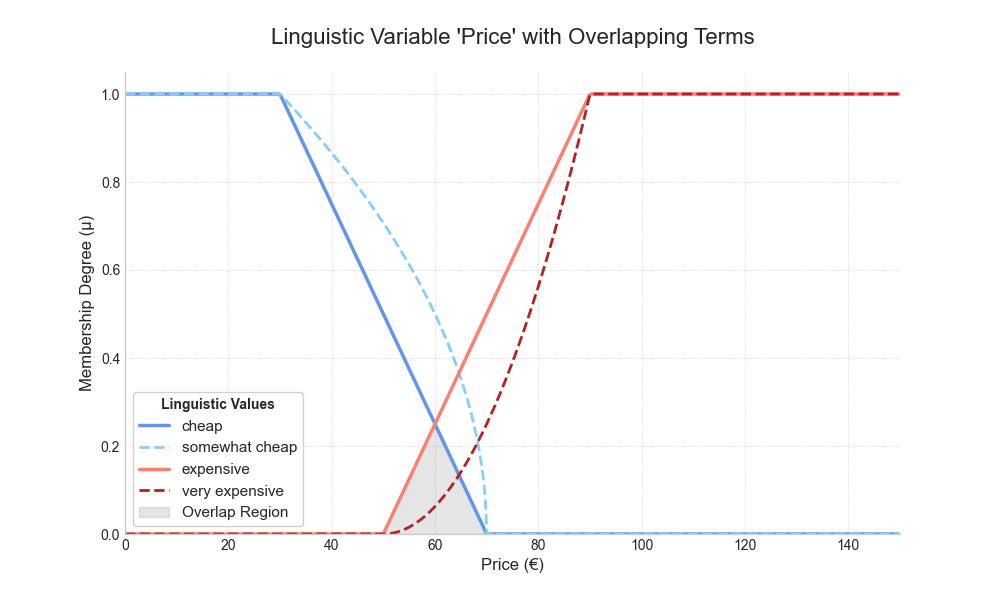
\includegraphics[width=0.8\textwidth]{ch2/figures/fuzzy_var_car_example.png}
    \caption{An illustration of the linguistic variable 'Price' with overlapping terms. The overlap between 'cheap' and 'expensive' represents the ambiguity of mid-range prices. Modifiers create more specific or general terms.}
    \label{fig:linguistic_variable_overlap}
\end{figure}


\subsection{Learning from Data}
When relevant data is available, membership functions can be constructed through learning algorithms. This approach frames the task as an optimization problem, where the goal is to find the membership function that best fit the available data.\\

In a supervised learning context, we have a dataset of input-output pairs. For example, consider a company with data regarding products (e.g. their characteristics) and customer satisfaction surveys. Each product would be an element of the universe and its membership grade is derived from the satisfaction surveys. We can then use function approximation techniques (e.g. Machine Learning models like artificial neural networks), to learn a membership function from the data and use them to generalize to new products with similar characteristics without needing to survey them.\\

In many real-world scenarios, however, we do not have such input-output pairs. For these unsupervised learning contexts, several approaches could be employed, such as fuzzy clustering (which is implemented in the next chapter). This algorithm partitions a dataset into several groups, allowing each data point to belong to multiple clusters with varying degrees of membership. These membership degrees can then be interpreted as the values of the membership function for the fuzzy set represented by each cluster. The Fuzzy C-Means (FCM) algorithm \cite{bezdek1984fcm} stands as the most widely used method in this category.

\paragraph{Fuzzy C-Means (FCM) algorithm} Given a dataset $X = \{x_1, x_2, \ldots, x_n\}$ of $n$ data points in an $r$-dimensional space, FCM aims to find a partition of $X$ into $c$ fuzzy clusters by minimizing the objective function:
\[
J_m(U, V) = \sum_{i=1}^{c} \sum_{k=1}^{n} (u_{ik})^m \|x_k - v_i\|^2
\]
where $U$ is the partition matrix with elements $u_{ik}$ representing the membership of data point $x_k$ in cluster $i$, $V = \{v_1, \ldots, v_c\}$ is the set of cluster centers, and $m > 1$ is a fuzzification parameter that controls the degree of cluster overlap. The minimization of $J_m$ is performed iteratively through the following steps:
\begin{enumerate}
    \item Initialize the partition matrix $U^{(0)}$ randomly, subject to $\sum_{i=1}^{c} u_{ik} = 1$ for each $k$.
    \item At iteration $t$, calculate the cluster centers $V^{(t)}$:
    \[
    v_i^{(t)} = \frac{\sum_{k=1}^{n} (u_{ik}^{(t-1)})^m x_k}{\sum_{k=1}^{n} (u_{ik}^{(t-1)})^m}
    \]
    \item Update the partition matrix $U^{(t)}$:
    \[
    u_{ik}^{(t)} = \left( \sum_{j=1}^{c} \left( \frac{\|x_k - v_i^{(t)}\|}{\|x_k - v_j^{(t)}\|} \right)^{\frac{2}{m-1}} \right)^{-1}
    \]
    \item Repeat steps 2 and 3 until the change in the partition matrix, $\|U^{(t)} - U^{(t-1)}\|$, is smaller than a predefined threshold.
\end{enumerate}
Once the algorithm converges, the resulting column $i$ of the matrix $U$ can be taken as the membership function for the fuzzy set represented by cluster $i$.\\

Memberships decay with the exponent ${-2/(m-1)}$, which provides key insights into the algorithm's operation. When $m$ approaches 1, the exponent approaches negative infinity, causing the nearest center to dominate and resulting in nearly crisp labels. Conversely, as $m$ approaches infinity, the exponent approaches 0, causing distances to lose influence and all memberships to converge to $1/c$. This behavior is clearly illustrated in Figure \ref{fig:fuzzy_cmeans}, which shows how different values of $m$ affect the clustering results.

\begin{figure}[!ht]
    \centering
    \begin{adjustwidth}{-1.7cm}{-1cm}
    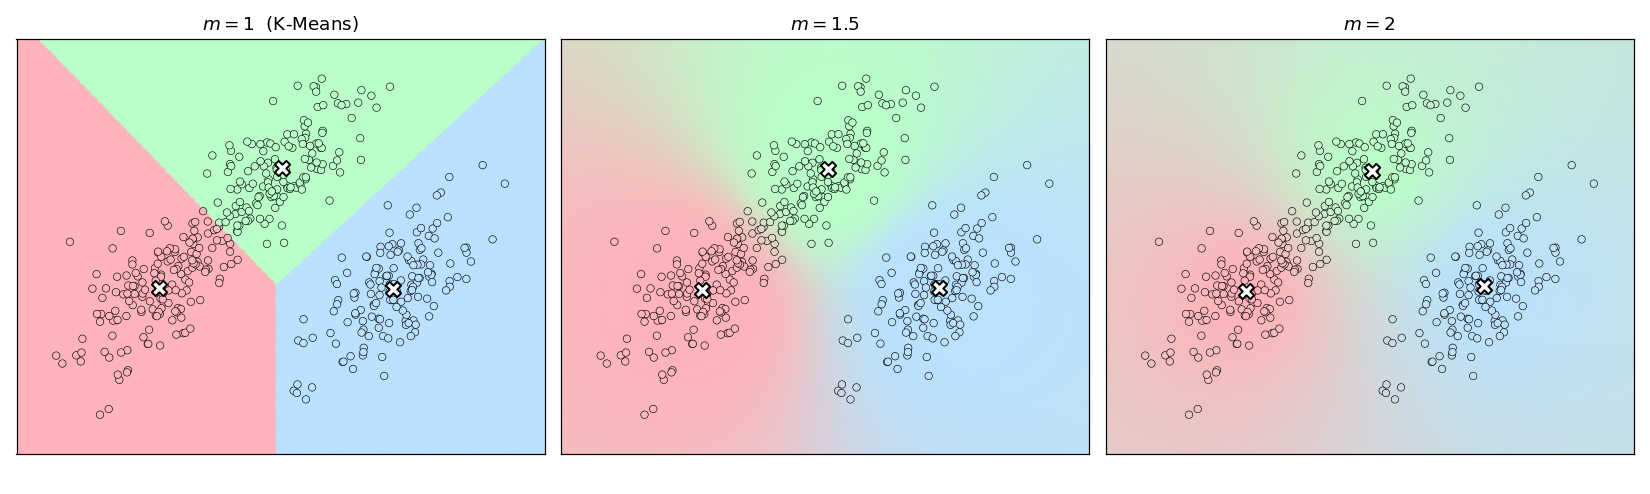
\includegraphics[width=1.15\textwidth]{ch2/figures/fuzzy_cmeans.png}
\end{adjustwidth}
    \caption{3 plots of fuzzy cmeans for 3 clusters with different m values (1, 1.5 and 2). Each color correspond to a cluster whose center is marked with the white cross. Memberships are denoted using gradients of color, where fainter tones denote lower membership values.}
    \label{fig:fuzzy_cmeans}
\end{figure}

\begin{example}
    A marketing firm could use FCM to segment customers based on their purchasing habits (e.g., purchase frequency and average transaction value). The algorithm might identify three clusters, like \emph{Low-Value}, \emph{Medium-Value}, and \emph{High-Value} customers. The membership value $u_{ik}$ would represent the degree to which customer $k$ belongs to the \emph{High-Value} fuzzy set, providing a more nuanced classification than a crisp assignment.
\end{example}

\subsection{Deriving from Other Fuzzy Sets}
New fuzzy sets can also be constructed from existing ones. The most common method is the use of fuzzy set operations (intersection, union and complement), which are particularly useful for creating complex fuzzy concepts from simpler, elementary ones. For instance, if we have already defined membership functions for the fuzzy sets \emph{cheap cars} and \emph{comfortable cars}, we can derive the membership function for \emph{cheap and comfortable cars} by applying a fuzzy AND operator (a t-norm) to the membership values of the original sets.\\

Another, more complex, method involves the use of fuzzy relational equations \cite[Sec.~3.5]{HistoryFL2017}. This approach is typically formulated as an inverse problem. A fuzzy relational equation describes a relationship between two or more fuzzy variables, often in the form $R = P \circ Q$, where $P$ and $Q$ are fuzzy relations and $\circ$ is a composition operator. If two of the three components are known, the third can be determined by solving the equation.

\begin{example}
    In medical diagnosis, let $S$ be a fuzzy relation between patients and symptoms, and $D$ be a fuzzy relation between patients and diseases. These two may be linked through a fuzzy relation $K$ representing medical knowledge, such that $D = S \circ K$. If we have observed data for patients' symptoms $S$ and their final diagnoses $D$, we could solve this equation to infer the underlying medical knowledge relation $K$ that connects symptoms to diseases.
\end{example}
\section{Fuzzy Aggregation}
Para qué usamos en el MDCM el fuzzy? Para manejar Uncertainty y subjectivity.

Information integration (aggregation)

Distance measures

Preference relations


\signal{OWA operators, y sus generalizaciones. Orness, andness, orlike y andlike.

Entropía de un OWA, quantifiers

Fuzzy implication operators para la importancia de los OWA

Fuzzy ratings, que es como tener 2 fuzzy weights y así incorporas la linguistic variable.

Fuzzy reasoning: tienes fuzzy rules y las agregas con un OWA por ejemplo. Puedes hacer la implicación y luego agregar o agregar y luego hacer la implicación.

MICA operators es la clase más general de operators en fuzzy modeling.

3 mecanismos de MISO fuzzy system

Compositional rule of inference

Generalized method of case inference rule

Interdependencia de los criterios!}

% \section{Fuzzy Preference Relations}
% \signal{Crea fuzzy additive preference relation o fuzzy multiplicative preference relation con lo que saca una judgement matrix en lugar de la decision matrix. Esto puede implementarse en algoritmos tipo AHP.}
% \section{Fuzzy Measure}

% \signal{Entropy measures o correlation measures para hacer un fuzzy clustering. También distance/similarity based measures between fuzzy elements para un fuzzy TOPSIS}

% \section{Other Approaches}
% \signal{Y si entendemos concepts como fuzzy sets, entonces buscamos relaciones entre concepts como fuzzy subsets (equiv fuzzy implications?) con un algoritmo tipo clustering y eso nos da información sobre los criterios que tenemos y cómo evalúan para cada alternative?\\
This way, we say that “$A$ is a fuzzy subset of $B$” if and only if

$I(\mu_A(x), \mu_B(x)) = 1$ for every $x$

And we can relax that condition to approximate fuzzy subset. Esto creo que se ha hecho ya con probabilistic reasoning.\\

Esto me recuerda mucho a lo que decía en Rough Sets y lo del trabajo de dominance based rough sets approach (DRSA) igual tiene ideas que se pueden llevar aquí. También estaba por ahí lo de DRSA con fuzzy para la inducción de reglas, eso puede estar muy bien.}